\documentclass[11pt]{article}
\usepackage{a4wide}
%\raggedright
%\usepackage{driverbook}
\usepackage{latexsym}           % math symbols that were omitted in latex2e
\usepackage{amsbsy}             % bold greek defs
\usepackage{amsmath,graphicx}
\usepackage{bbm}
\usepackage{mathrsfs}
\usepackage{stmaryrd}
\usepackage{graphics}
\usepackage{acronym}
\usepackage{longtable}
\usepackage{mathtools}
\usepackage{times}
\usepackage{setspace}
\usepackage{cite}
\usepackage{array}
\usepackage{subfigure}
\usepackage{amsmath,amsthm}
\usepackage{amssymb}
\usepackage{wasysym,url}
\usepackage{fixltx2e,amsmath}
\usepackage{setspace,float}
\usepackage{color}
\usepackage{cases,bm}
\usepackage{mathrsfs}
\usepackage{enumitem}
\usepackage{hyperref}
\usepackage{mathtools,cuted}
\usepackage[linesnumbered,ruled,vlined]{algorithm2e}
\usepackage{epsfig}
\usepackage{color}
\DontPrintSemicolon

\usepackage{geometry}
 \geometry{
 a4paper,
 total={170mm,257mm},
 left=20mm,
 top=30mm,
 bottom=30mm,
 }
 
 
\usepackage{listings}
\usepackage{xcolor}

\definecolor{codegreen}{rgb}{0,0.6,0}
\definecolor{codegray}{rgb}{0.5,0.5,0.5}
\definecolor{codepurple}{rgb}{0.58,0,0.82}
\definecolor{backcolour}{rgb}{0.95,0.95,0.92}

\lstdefinestyle{mystyle}{
    backgroundcolor=\color{backcolour},   
    commentstyle=\color{codegreen},
    keywordstyle=\color{magenta},
    numberstyle=\tiny\color{codegray},
    stringstyle=\color{codepurple},
    basicstyle=\ttfamily\footnotesize,
    breakatwhitespace=false,         
    breaklines=true,                 
    captionpos=b,                    
    keepspaces=true,                 
    numbers=left,                    
    numbersep=5pt,                  
    showspaces=false,                
    showstringspaces=false,
    showtabs=false,                  
    tabsize=2
}

\lstset{style=mystyle}

\newcommand{\by}{\mathbf{y}}
\newcommand{\br}{\mathbf{r}}
\newcommand{\ba}{\mathbf{a}}
\newcommand{\bh}{\mathbf{h}}
\newcommand{\bx}{\mathbf{x}}
\newcommand{\bs}{\mathbf{s}}
\newcommand{\bw}{\mathbf{w}}
\newcommand{\bR}{\mathbf{R}}
\newcommand{\bI}{\mathbf{I}}
\newcommand{\bA}{\mathbf{A}}
\newcommand{\bH}{\mathbf{H}}
\newcommand{\bQ}{\mathbf{Q}}
\newcommand{\bG}{\mathbf{G}}
\newcommand{\bC}{\mathbf{C}}
\newcommand{\rr}{\mathbb{R}}
\newcommand{\zz}{\mathbb{Z}}
\newcommand{\nn}{\mathbb{N}}
\newcommand{\cc}{\mathbb{C}}
\newcommand{\Ex}{\mathbb{E}}
\newcommand{\TT}{\mathsf{T}}
\newcommand{\HH}{\mathsf{H}}
\newcommand{\cH}{\mathcal{H}}
\newcommand{\dd}{\mathrm{d}}
\newcommand{\jj}{\mathrm{j}}

\newcommand{\zerovec}{\boldsymbol{0}}
\newcommand{\bSigma}{\boldsymbol{\Sigma}}
\newcommand{\btheta}{\boldsymbol{\theta}}
\newcommand{\bgamma}{\boldsymbol{\gamma}}

\begin{document}
\thispagestyle{empty}

{\small
\begin{flushleft}
   Name: Abijith J. Kamath\\
   Student Id: 17788
\end{flushleft}
}
\vspace{2ex}
\begin{center}
    {\Large\bf E1 244: Detection and Estimation}\\
    February-May 2021

\vspace{5mm}
{\bf Solution -- Homework 3}
\end{center}
\vspace{5mm}

\section*{Analysis and Algorithms for Spectrum Sensing in Cognitive Radio}

% -----------------------------------------------------------------------------------------------------------------------
% -----------------------------------------------------------------------------------------------------------------------

\subsection*{Part A: Derivation and Modelling}
\label{subsec:partA}

Consider the OFDM transmission of the sequence $s$ of length $N_{d}$, where the $N_{d}$-point IFFT of the sequence along with an $N_{c}$ length cyclic prefix is transmitted over an AWGN channel. The transmitted sequence is defined using:
\begin{equation}
	x[n] = \frac{1}{\sqrt{N_{d}}} \sum_{k=0}^{N_{d}-1} s[k] e^{\jj 2\pi nk/N_{d}}, \; n=0,1,\cdots, N_{d}-1,
\label{eq:transmittedSignal}
\end{equation}
The transmitted vector has entries defined by $x[n]$ with the last $N_{c}$ points are prefixed to itself to form an $N_{d}+N_{c}$ length transmission vector $\bx_{i} = \left[ x[0] \; x[1] \; \cdots \; x[N_{d}+N_{c}-1] \right]^{\TT}$. This forms one OFDM symbol block. $K+1$ such OFDM symbol blocks $\bx = [\bx_{0}^{\TT} \; \bx_{1}^{\TT} \; \cdots \; \bx_{K}^{\TT}]^{\TT}$ are transmitted over an AWGN channel to give measurements $\by = \bx + \bw$, where $\bw \sim \mathcal{N}(\zerovec, \sigma_{w}^{2} \mathbf{I})$.

% -----------------------------------------------------------------------------------------------------------------------

\subsubsection*{Energy Detector}
\label{subsubsec:energyDetector}

Consider the data symbols $\bs = \left[ s[0] \; s[1] \; \cdots \; s[N_{d}-1] \right]^{\TT}$ where the entries are QPSK with variance $\sigma_{s}^{2} = 1$, i.e., $s[k] \in \{ \pm 1/\sqrt{2} \pm \jj 1/\sqrt{2} \}$. Suppose the number of data points $N_{d}$ is large, using the central limit theorem, the OFDM symbol blocks $\bx_{i}$ can be assumed to be zero-mean Gaussians with identity covariance of size $(K+1)(N_{d}+N_{c})$ as $\Ex[\bx_{i} \bx_{i}^{\HH}] = \sigma_{s}^{2} \mathbf{I}$.

Given measurements $\by \in \cc^{(K+1)(N_{d}+N_{c})}$, the signal detection problem is to select between one of the two following hypothesis:
\begin{equation}
\begin{split}
	\mathcal{H}_{0}: \by &= \bw, \\
	\mathcal{H}_{1}: \by &= \bx + \bw.
\end{split}
\label{eq:detectionProblem}
\end{equation}
The Neymann-Pearson detector uses the likelihood ratio test (LRT). Let the measurements have the density function $p_{Y}(\by ; \cH_{0})$ and $p_{Y}(\by ; \cH_{1})$ under the hypothesis $\cH_{0}$ and $\cH_{1}$ respectively. The LRT compares the ratio of the likelihoods to a threshold, and decides on the hypothesis $\cH_{1}$ if:
\begin{equation}
\begin{split}
L(\by) &= \frac{p_{Y}(\by ; \cH_{1})}{p_{Y}(\by ; \cH_{0})} > \gamma, \\
&= \frac{\frac{1}{(2\pi(\sigma_{s}^{2} + \sigma_{w}^{2}))^{N/2}} \mathrm{exp}\left(-\frac{1}{2(\sigma_{s}^{2}+\sigma_{w}^{2})} \sum_{n=0}^{N}\vert y[n] \vert^{2} \right)}{\frac{1}{(2\pi\sigma_{w}^{2})^{N/2}} \mathrm{exp}\left(-\frac{1}{2\sigma_{w}^{2}} \sum_{n=0}^{N}\vert y[n] \vert^{2} \right)}, \\
&= \left(\frac{\sigma_{w}^{2}}{\sigma_{s}^{2}+\sigma_{w}^{2}}\right)^{N/2} \mathrm{exp} \left( \frac{1}{2} \frac{\sigma_{s}^{2}}{\sigma_{w}^{2}(\sigma_{s}^{2}+\sigma_{w}^{2})} \sum_{n=0}^{N-1} \vert y[n] \vert^{2} \right), \\
\implies T(\by) &= \sum_{n=0}^{N-1} \vert y[n] \vert^{2} > \gamma'.
\end{split}
\label{eq:energyLRT}
\end{equation}
where $N = N_{d}+N_{c}$ and $\gamma'$ is a threshold that is set by $P_{FA}$. The test statistic $T(\by)$ is the square of sum of Gaussian random variables and hence, has the chi-squared distribution. The hypotheses with this test statistic are:
\begin{equation}
\begin{split}
	\mathcal{H}_{0}&: \frac{T(\by)}{\sigma_{w}^{2}} \sim \chi^{2} \\
	\mathcal{H}_{1}&: \frac{T(\by)}{\sigma_{w}^{2} + \sigma_{s}^{2}} \sim \chi^{2}.
\end{split}
\label{eq:hypothesesEnergy}
\end{equation}
The probability of false alarm, $P_{FA} = p_{Y}(T(\by)>\gamma' ; \cH_{0}) = Q(\frac{\gamma'}{\sigma_{w}^{2}})$, where $Q(\cdot)$ is the CDF of the chi-squared distribution with $N$ degrees of freedom. Hence, given a choice for $P_{FA}$, the threshold can be computed as $\gamma' = \sigma_{w}^{2} Q^{-1}(P_{FA})$. Using this, the probability of detection:
\begin{equation}
\begin{split}
	P_{D} &= p_{Y}(T(\by)>\gamma';\cH_{1}), \\
	&= Q\left(\frac{\gamma'}{\sigma_{w}^{2} + \sigma_{s}^{2}}\right).
\end{split}
\label{eq:probDetectionEnergy}
\end{equation}

% -----------------------------------------------------------------------------------------------------------------------

\subsubsection*{Cyclostationarity Detector}
\label{subsubsec:cyclostationarityDetector}

Under the same transmission settings, consider test function for LRT defined as:
\begin{equation}
\begin{split}
	T(\by) &= \sum_{n=0}^{N_{c}-1} \hat{R}[n], \\
	&= \sum_{n=0}^{N_{c}-1} \frac{1}{K} \sum_{k=0}^{K-1} \hat{r}[n+k(N_{c}+N_{d}), N_{d}], \\
	&= \frac{1}{K} \sum_{n=0}^{N_{c}-1}\sum_{k=0}^{K-1} y[n+k(N_{c}+N_{d})] y^{*}[n+k(N_{c}+N_{d})+N_{d}].
\end{split}
\label{eq:cycTest}
\end{equation}
Suppose the number of data samples are high, using the central limit theorem, the test statistic $T(\by)$ can be taken to be a complex Gaussian random variable.

\noindent \linebreak {\it a) Distribution of the test statistic:} Let $T(\by) = \bar{T}(\by) + \jj \tilde{T}(\by)$ be defined as in (\ref{eq:cycTest}) be approximated as a complex Gaussian random variable.

Under $\cH_{0}$, $\by = \bw$, i.e., $y[m] = w[m], \; \forall m$. Therefore, $\Ex\left[ y[n+kN] y^{*}[n+kN+N_{d}] \right] \break = \Ex\left[ w[n+kN] w^{*}[n+kN+N_{d}] \right] = 0$.
\begin{equation}
\begin{split}
	\Ex[T(\by)] &= \frac{1}{K} \sum_{n=0}^{N_{c}-1}\sum_{k=0}^{K-1} \Ex \left[y[n+kN] y^{*}[n+kN+N_{d}]\right], \\
	&= 0, \\
	\implies \Ex[\bar{T}(\by)] &= \Ex[\tilde{T}(\by)] = 0.
\end{split}
\label{eq:meanH0}
\end{equation}
To find the variance, consider the equations for $T^{2}(\by) = \bar{T}^{2}(\by) + \jj 2\bar{T}(\by)\tilde{T}(\by) - \tilde{T}^{2}(\by)$ and $\vert T(\by) \vert^{2} = \bar{T}^{2}(\by) + \tilde{T}^{2}(\by)$.
\begin{equation}
\begin{split}
	T^{2}(\by) = \frac{1}{K^{2}} \sum_{n_{1}=0}^{N_{c}-1} \sum_{k_{1}=0}^{K-1} \sum_{n_{2}=0}^{N_{c}-1} \sum_{k_{2}=0}^{K-1} & y[n_{1}+k_{1}N] y^{*}[n_{1}+k_{1}N+N_{d}] \\ & y[n_{2}+k_{2}N] y^{*}[n_{2}+k_{2}N+N_{d}].
\end{split}
\label{eq:statSquared}
\end{equation}
We have, $\Ex \left[ y[n_{1}+k_{1}N] y^{*}[n_{1}+k_{1}N+N_{d}] y[n_{2}+k_{2}N] y^{*}[n_{2}+k_{2}N+N_{d}] \right] \break = \Ex\left[ w[n_{1}+k_{1}N] w^{*}[n_{1}+k_{1}N+N_{d}] w[n_{2}+k_{2}N] w^{*}[n_{2}+k_{2}N+N_{d}] \right] = \sigma_{w}^{4}\delta(n_{1}-n_{2},k_{1}-k_{2})$, and hence:
\begin{equation}
	\Ex\left[ T^{2}(\by) \right] = \frac{1}{K^{2}} N_{c}K\sigma_{w}^{4} = \frac{1}{K} N_{c}\sigma_{w}^{4}.
\label{eq:comVarH0}
\end{equation}
Since the quantity is real, $\Ex\left[\bar{T}(\by)\tilde{T}(\by)\right] = \mathrm{cov}\left(\bar{T}(\by),\tilde{T}(\by)\right) = 0$. Since the measurements are noise-only and real, $\Ex\left[ \vert T(\by) \vert^{2} \right] = \Ex\left[ T^{2}(\by) \right] = \frac{1}{K} N_{c}\sigma_{w}^{4}$. Using this and (\ref{eq:comVarH0}):
\begin{equation}
\begin{split}
	\mathrm{var}\left( \bar{T}(\by) \right) = \mathrm{var}\left( \tilde{T}(\by) \right) = \frac{1}{2K} N_{c}\sigma_{w}^{4}.
\end{split}
\label{eq:VarH0}
\end{equation}

Under $\cH_{1}$, $\by = \bx + \bw$, i.e., $y[m] = x[m] + w[m], \; \forall m$. Therefore, $\Ex\left[ y[n+kN] y^{*}[n+kN+N_{d}] \right] =  \Ex\left[ \left(x[n+kN] + w[n+kN]\right) \left(x[n+kN+N_{d}] + w[n+kN+N_{d}]\right)^{*} \right] = \sigma_{s}^{2} = 1$.
\begin{equation}
\begin{split}
	\Ex[T(\by)] &= \frac{1}{K} \sum_{n=0}^{N_{c}-1}\sum_{k=0}^{K-1} \Ex \left[y[n+kN] y^{*}[n+kN+N_{d}]\right], \\
	&= \frac{1}{K} N_{c}K = N_{c}, \\
	\implies \Ex[\bar{T}(\by)] &= N_{c}, \\
	\Ex[\tilde{T}(\by)] &= 0,
\end{split}
\label{eq:meanH1}
\end{equation}
since $\Ex[T(\by)]$ is real. To find the variance, similar to the case in $\cH_{0}$, using (\ref{eq:statSquared}), we have:
\begin{equation*}
\begin{split}
&\Ex \left[ y[n_{1}+k_{1}N] y^{*}[n_{1}+k_{1}N+N_{d}] y[n_{2}+k_{2}N] y^{*}[n_{2}+k_{2}N+N_{d}] \right] = \\
&\Ex [\left(x[n_{1}+k_{1}N] + w[n_{1}+k_{1}N]\right) \left(x[n_{1}+k_{1}N+N_{d}] + w[n_{1}+k_{1}N+N_{d}]\right)^{*} \\
&\left(x[n_{2}+k_{2}N] + w[n_{2}+k_{2}N]\right) \left(x[n_{2}+k_{2}N+N_{d}] + w[n_{2}+k_{2}N+N_{d}]\right)^{*}] = \begin{cases}
	\sigma_{s}^{4}, & n_{1} \neq n_{2}, k_{1} \neq k_{2}, \\
	\sigma_{s}^{4} + \sigma_{s}^{4}, & n_{1} = n_{2}, k_{1} = k_{2},
\end{cases}
\end{split}
\end{equation*}
and hence:
\begin{equation}
	\Ex\left[ T^{2}(\by) \right] = \frac{1}{K^{2}} \left( 2N_{c}K + N_{c}^{2}K^{2} - N_{c}K \right) = N_{c}^{2} + \frac{N_{c}}{K}.
\label{eq:comVarH1}
\end{equation}
Since the quantity is real, $\Ex\left[\bar{T}(\by)\tilde{T}(\by)\right] = \mathrm{cov}\left(\bar{T}(\by),\tilde{T}(\by)\right) = 0$. In this case, the measurements are not all real. Hence:
\begin{equation}
\begin{split}
	\vert T(\by) \vert^{2} = \frac{1}{K^{2}} \sum_{n_{1}=0}^{N_{c}-1} \sum_{k_{1}=0}^{K-1} \sum_{n_{2}=0}^{N_{c}-1} \sum_{k_{2}=0}^{K-1} & y[n_{1}+k_{1}N] y^{*}[n_{1}+k_{1}N+N_{d}] \\ & y^{*}[n_{2}+k_{2}N] y[n_{2}+k_{2}N+N_{d}],
\end{split}
\label{eq:statSquared}
\end{equation}
with the mean of each term in the sum:
\begin{equation*}
\begin{split}
&\Ex \left[ y[n_{1}+k_{1}N] y^{*}[n_{1}+k_{1}N+N_{d}] y^{*}[n_{2}+k_{2}N] y[n_{2}+k_{2}N+N_{d}] \right] = \\
&\Ex [\left(x[n_{1}+k_{1}N] + w[n_{1}+k_{1}N]\right) \left(x[n_{1}+k_{1}N+N_{d}] + w[n_{1}+k_{1}N+N_{d}]\right)^{*} \\
&\left(x[n_{2}+k_{2}N] + w[n_{2}+k_{2}N]\right)^{*} \left(x[n_{2}+k_{2}N+N_{d}] + w[n_{2}+k_{2}N+N_{d}]\right)] \\
&= \begin{cases}
	\sigma_{s}^{4}, & n_{1} \neq n_{2}, k_{1} \neq k_{2}, \\
	2\sigma_{s}^{4} + 2\sigma_{s}^{2}\sigma_{w}^{2} + \sigma_{w}^{4}, & n_{1} = n_{2}, k_{1} = k_{2},
\end{cases}
\end{split}
\end{equation*}
and hence,
\begin{equation}
	\Ex\left[ \vert T(\by) \vert^{2} \right] = N_{c}^{2} + \frac{N_{c}}{K}\left( 1 + 2\sigma_{w}^{2} + \sigma_{w}^{4} \right).
\label{eq:comAbsVarH1}
\end{equation}
Using (\ref{eq:comVarH1}) and (\ref{eq:comAbsVarH1}):
\begin{equation}
\begin{split}
	\mathrm{var}\left( \bar{T}(\by) \right) &= N_{c}^{2} + \frac{N_{c}}{K}\left( 1 + \sigma_{w}^{2} + \frac{\sigma_{w}^{4}}{2} \right), \\
	\mathrm{var}\left( \tilde{T}(\by) \right) &= \frac{N_{c}}{K}\left(\sigma_{w}^{2} + \frac{\sigma_{w}^{4}}{2} \right).
\end{split}
\label{eq:VarH1}
\end{equation}

\noindent \linebreak {\it b) Neymann-Pearson detector:} Using the test statistic defined in (\ref{eq:cycTest}), the detector chooses hypotheses $\cH_{1}$ if $\vert T(\by) \vert > \gamma$ or equivalently, $\vert T(\by) \vert^{2} > \gamma^{2}$. The probability of false alarm:
\begin{equation}
\begin{split}
	P_{FA} &= p_{Y}(\vert T(\by) \vert^{2} > \gamma^{2}) ; \cH_{0}), \\
	&= p_{Y}(\bar{T}^{2}(\by) + \tilde{T}^{2}(\by) > \gamma^{2}) ; \cH_{0}), \\
	&= Q \left( \frac{\gamma^{2}}{\frac{N_{c}}{2K}\sigma_{w}^{4}} \right),
\end{split}
\label{eq:cycPfa}
\end{equation}
where $Q(\cdot)$ is the CDF of the chi-squared distribution with $2$ degrees of freedom. Therefore, given a choice for the probability of false alarm, the threshold is chosen as:
\begin{equation}
	\gamma = \left( \frac{N_{c}}{2K}\sigma_{w}^{4} Q^{-1}(P_{FA}) \right)^{1/2}.
\label{eq:cycThresh}
\end{equation}


% -----------------------------------------------------------------------------------------------------------------------
% -----------------------------------------------------------------------------------------------------------------------

\subsection*{Part B: Implementation}
\label{subsec:partB}


% -----------------------------------------------------------------------------------------------------------------------

\subsubsection*{Energy Detector}
\label{subsubsec:energyDetectorImplementation}

\noindent {\it a) Monte-Carlo simulations with exact parameters:}

Figures \ref{fig:EDPD} and \ref{fig:EDPFA} shows the variation of $P_{D}$ and $P_{FA}$ with the signal-to-noise ratio (SNR). The estimated results are averaged over $1000$ realisations of the test statistic. The estimated probability and the theoretical probability match up to numerical precision. It can observed that the probability of detection increases monotonically with increase in SNR. High probabilities of detection $>0.9$ are achieved with SNR $>-10$dB. The estimated probability of false alarm is consistent to be around the true value of $0.05$.
\begin{figure}[h]
\centering
\subfigure[Probability of detection.]{\label{fig:EDPD}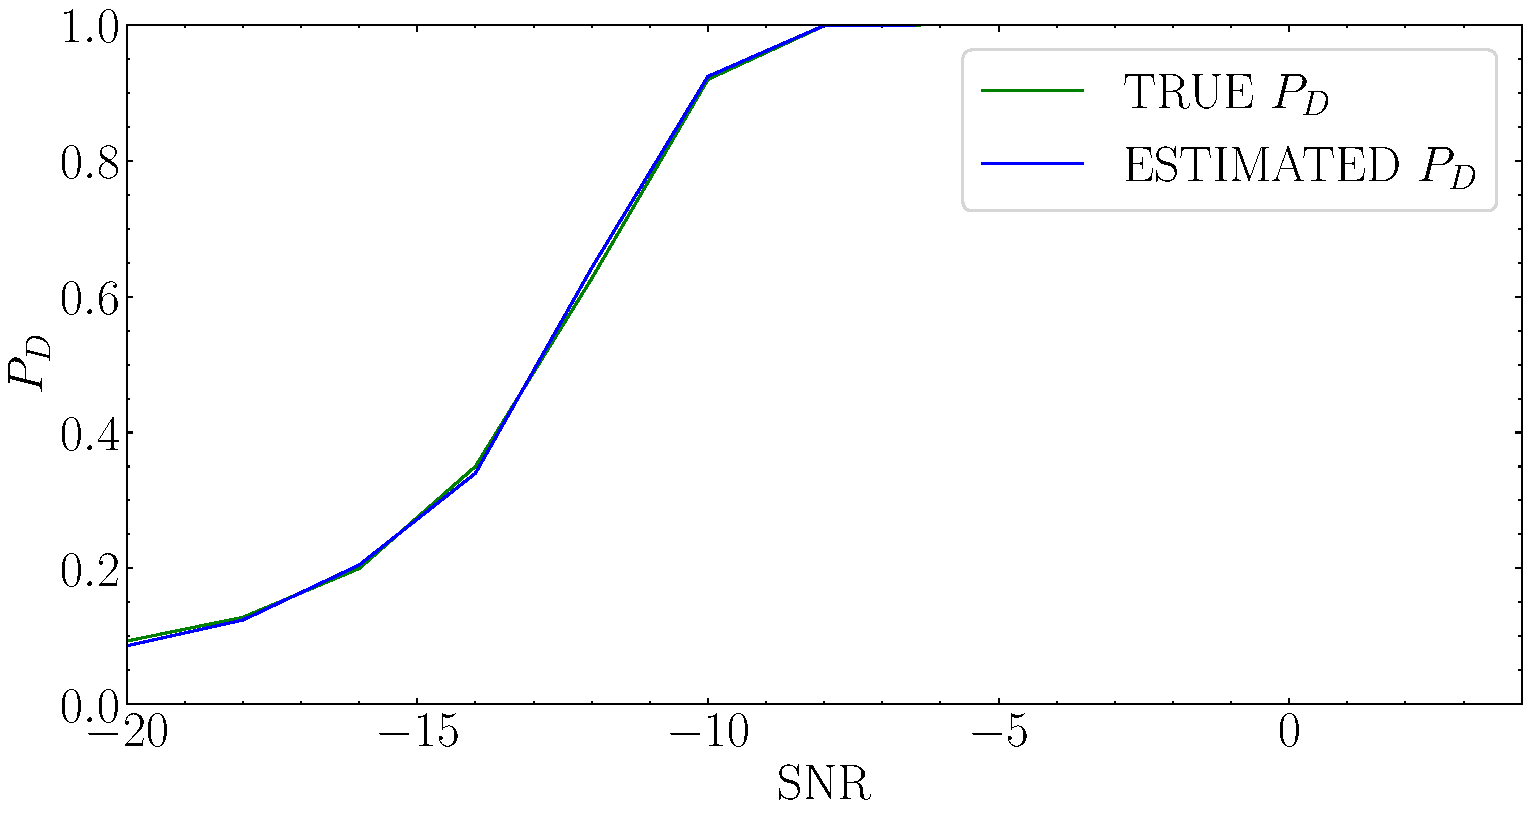
\includegraphics[width=3in]{../results/eneProb_PD}}
\subfigure[Probability of false alarm.]{\label{fig:EDPFA}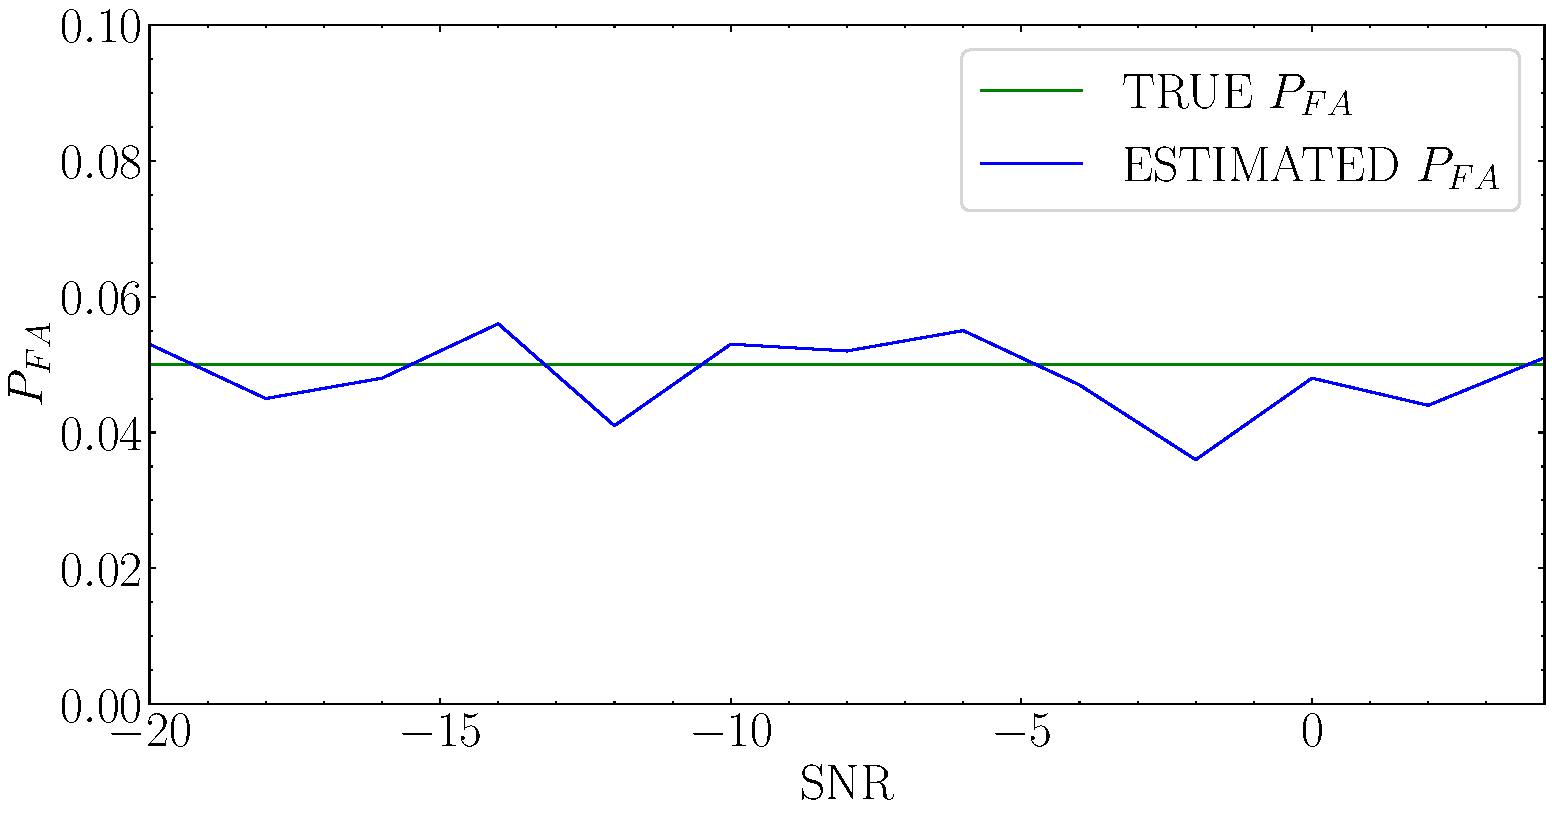
\includegraphics[width=3in]{../results/eneProb_PFA}}
\caption{Monte-Carlo probabilities of the energy detector varying with SNR when the parameters are exact.}
\label{fig:ED_exact}
\end{figure}

\noindent \linebreak {\it b) Monte-Carlo simulations with inexact parameters:}

Figures \ref{fig:EDPD_noise} and \ref{fig:EDPFA_noise} shows the variation of $P_{D}$ and $P_{FA}$ with the signal-to-noise ratio (SNR). The estimated results are averaged over $1000$ realisations of the test statistic. As compared to Figures \ref{fig:EDPD} and \ref{fig:EDPFA}, the probability of detection is only as high as $0.8$ at the SNR of $-10$dB. The probability of false alarm is also consistently higher than the true value.
\begin{figure}[t]
\centering
\subfigure[Probability of detection.]{\label{fig:EDPD_noise}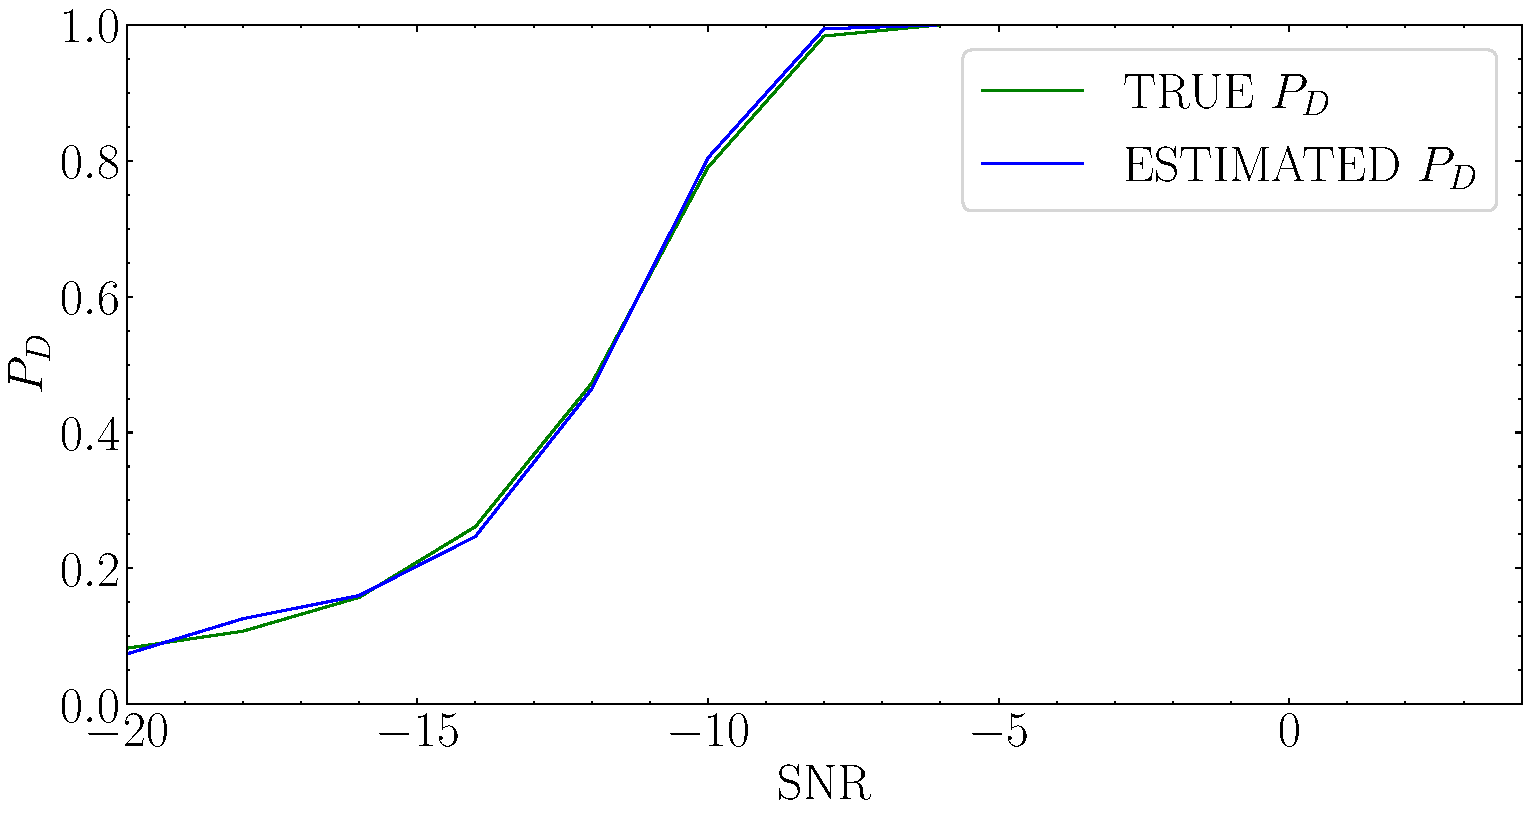
\includegraphics[width=3in]{../results/eneProb_PD_Noisy}}
\subfigure[Probability of false alarm.]{\label{fig:EDPFA_noise}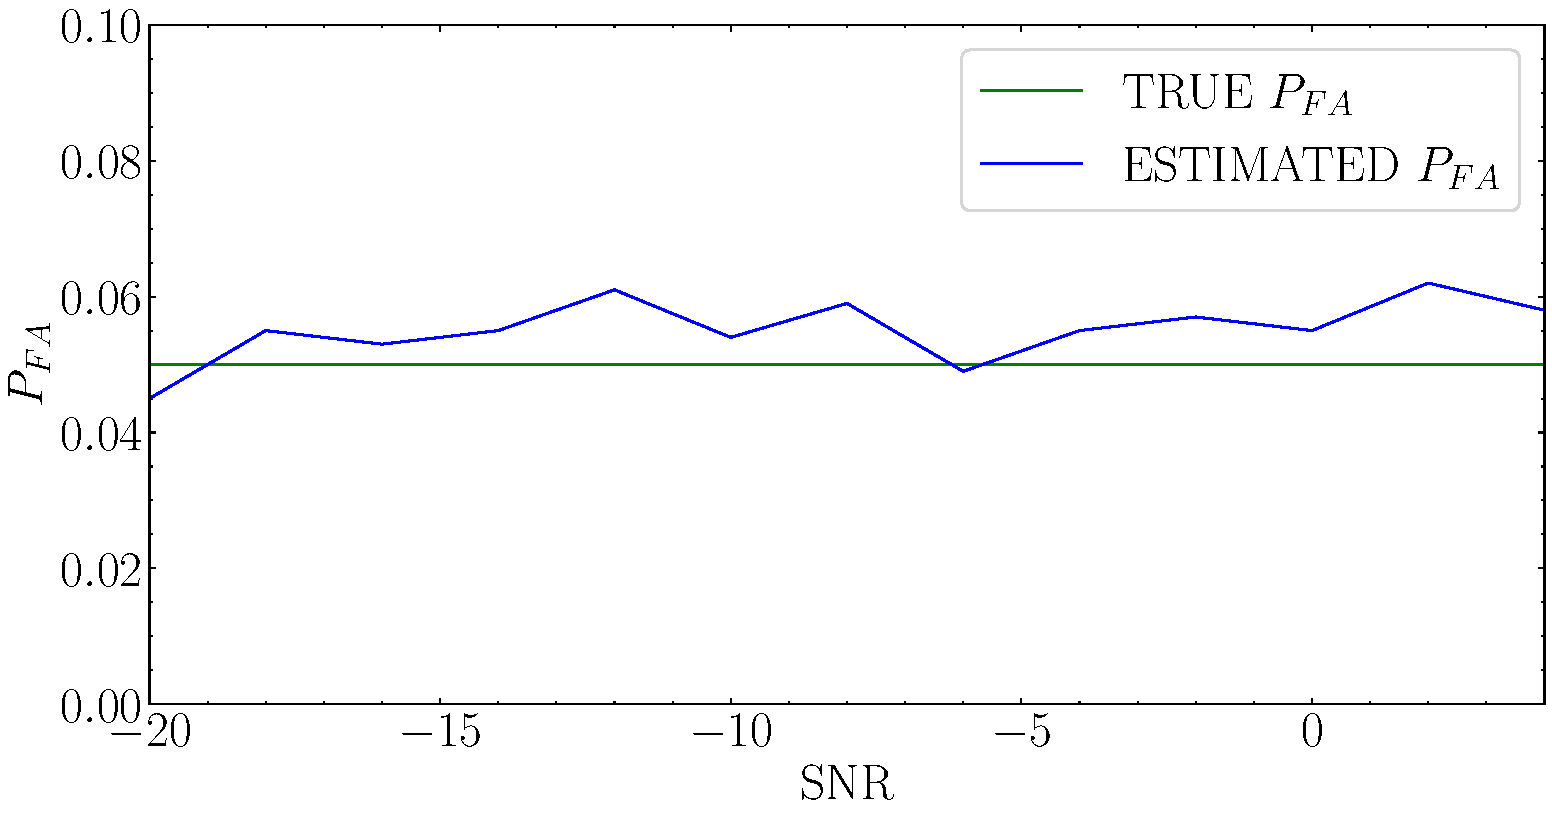
\includegraphics[width=3in]{../results/eneProb_PFA_Noisy}}
\caption{Monte-Carlo probabilities of the energy detector varying with SNR when the parameters are inexact.}
\label{fig:ED_inexact}
\end{figure}

\noindent \linebreak {\it c) Comparison with the Bayes' detector:} The Bayes' detector, similar to the LRT, compares the ratio of the likelihoods to the ratio of the prior probabilities. The Bayes' detector decides on $\cH_{1}$ if:
\begin{equation}
\begin{split}
L(\by) &= \frac{p_{Y}(\by ; \cH_{1})}{p_{Y}(\by ; \cH_{0})} > \frac{P[\cH_{0}]}{P[\cH_{1}]}, \\
&= \frac{\frac{1}{(2\pi(\sigma_{s}^{2} + \sigma_{w}^{2}))^{N/2}} \mathrm{exp}\left(-\frac{1}{2(\sigma_{s}^{2}+\sigma_{w}^{2})} \sum_{n=0}^{N}\vert y[n] \vert^{2} \right)}{\frac{1}{(2\pi\sigma_{w}^{2})^{N/2}} \mathrm{exp}\left(-\frac{1}{2\sigma_{w}^{2}} \sum_{n=0}^{N}\vert y[n] \vert^{2} \right)} > \frac{P[\cH_{0}]}{P[\cH_{1}]} \\
&= \left(\frac{\sigma_{w}^{2}}{\sigma_{s}^{2}+\sigma_{w}^{2}}\right)^{N/2} \mathrm{exp} \left( \frac{1}{2} \frac{\sigma_{s}^{2}}{\sigma_{w}^{2}(\sigma_{s}^{2}+\sigma_{w}^{2})} \sum_{n=0}^{N-1} \vert y[n] \vert^{2} \right) > \frac{P[\cH_{0}]}{P[\cH_{1}]} \\
\implies T(\by) &= \sum_{n=0}^{N-1} \vert y[n] \vert^{2} > 2\left( \frac{(\sigma_{s}^{2}+\sigma_{w}^{2})\sigma_{w}^{2}}{\sigma_{s}^{2}} \right) \left( \frac{N}{2} \ln\left( \frac{\sigma_{s}^{2}+\sigma_{w}^{2}}{\sigma_{w}^{2}} \right) + \ln\left( \frac{P[\cH_{0}]}{P[\cH_{1}]} \right)\right).
\end{split}
\label{eq:energyBayes}
\end{equation}

Figure \ref{fig:thresholds} shows the variation of the thresholds of the Neymann-Pearson detector and the Bayes' detector with the SNR. It can be observed that the thresholds decrease monotonically with SNR as the energy in the noise decreases with increasing SNR, and a small threshold reliably detects the signal. Between the detectors, it can be observed that, for a probability of false alarm $P_{FA} = 0.05$ in the Neymann-Pearson detector and a prior $P[\cH_{0}] = 0.2$ in the Bayes' detector, the thresholds are similar. The threshold of the Neymann-Pearson detector is marginally smaller than the threshold of the Bayes' detector at lower SNR, and gradually meet as the SNR increases.
\begin{figure}[b]
\centering
	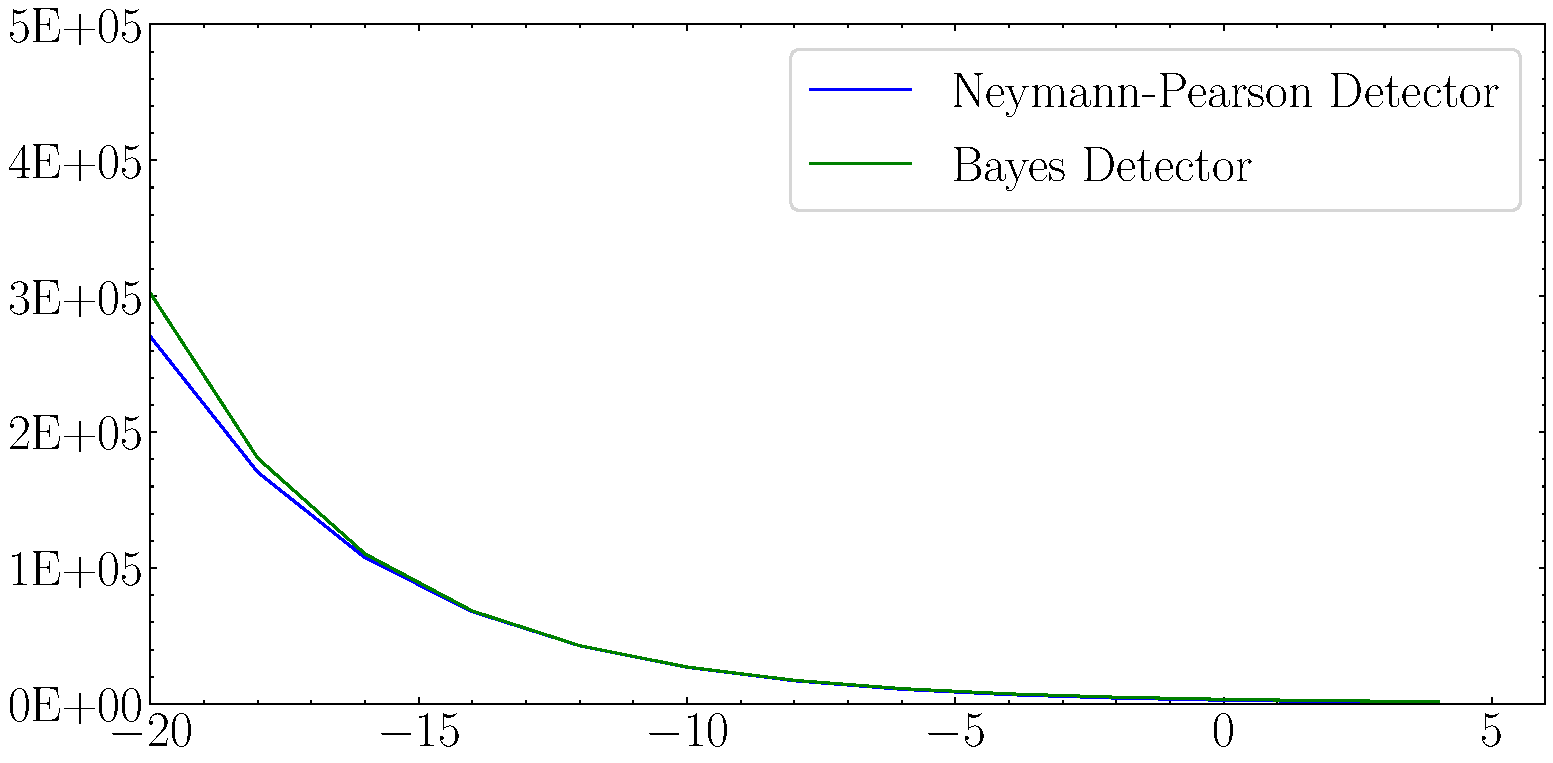
\includegraphics[width=3in]{../results/thresholds}
\caption{Variation of Neymann-Pearson threshold vs. Bayes' threshold with SNR.}
\label{fig:thresholds}
\end{figure}

% -----------------------------------------------------------------------------------------------------------------------

\subsubsection*{Cyclostationarity Detector}
\label{subsubsec:cyclostationarityDetectorImplementation}

\noindent \linebreak {\it a) Distribution of the test statistics:}

Figures \ref{fig:CD_H0R} and \ref{fig:CD_H0I} shows the real and imaginary parts of the density function of the test statistic under $\cH_{0}$, and Figures \ref{fig:CD_H1R} and \ref{fig:CD_H1I} shows the real and imaginary parts of the density function of the test statistic under $\cH_{1}$. The histogram is plotted using $1000$ realisation of each test statistic, and is compared with the Gaussian PDF with parameters derived. The approximation is known to improve with longer data samples $N_{d}$. With $N_{d}=32$ and $K=50$, the distributions are fairly well approximated by a Gaussian random variable.
\begin{figure}[h]
\centering
\subfigure[Real component in $\cH_{0}$.]{\label{fig:CD_H0R}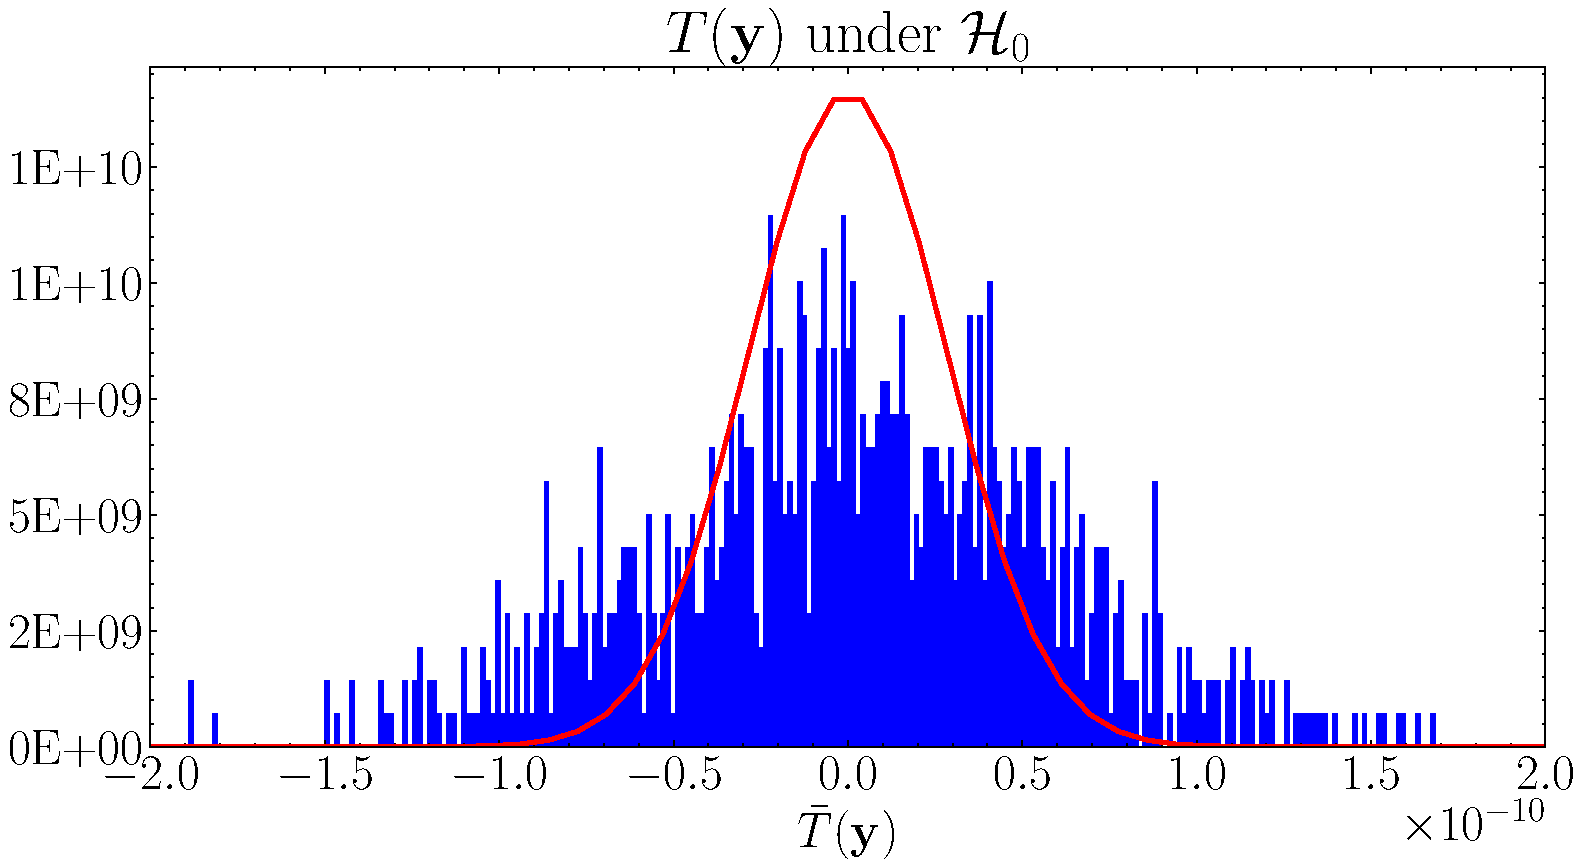
\includegraphics[width=3in]{../results/cycDist_H0R}}
\subfigure[Imaginary component in $\cH_{0}$.]{\label{fig:CD_H0I}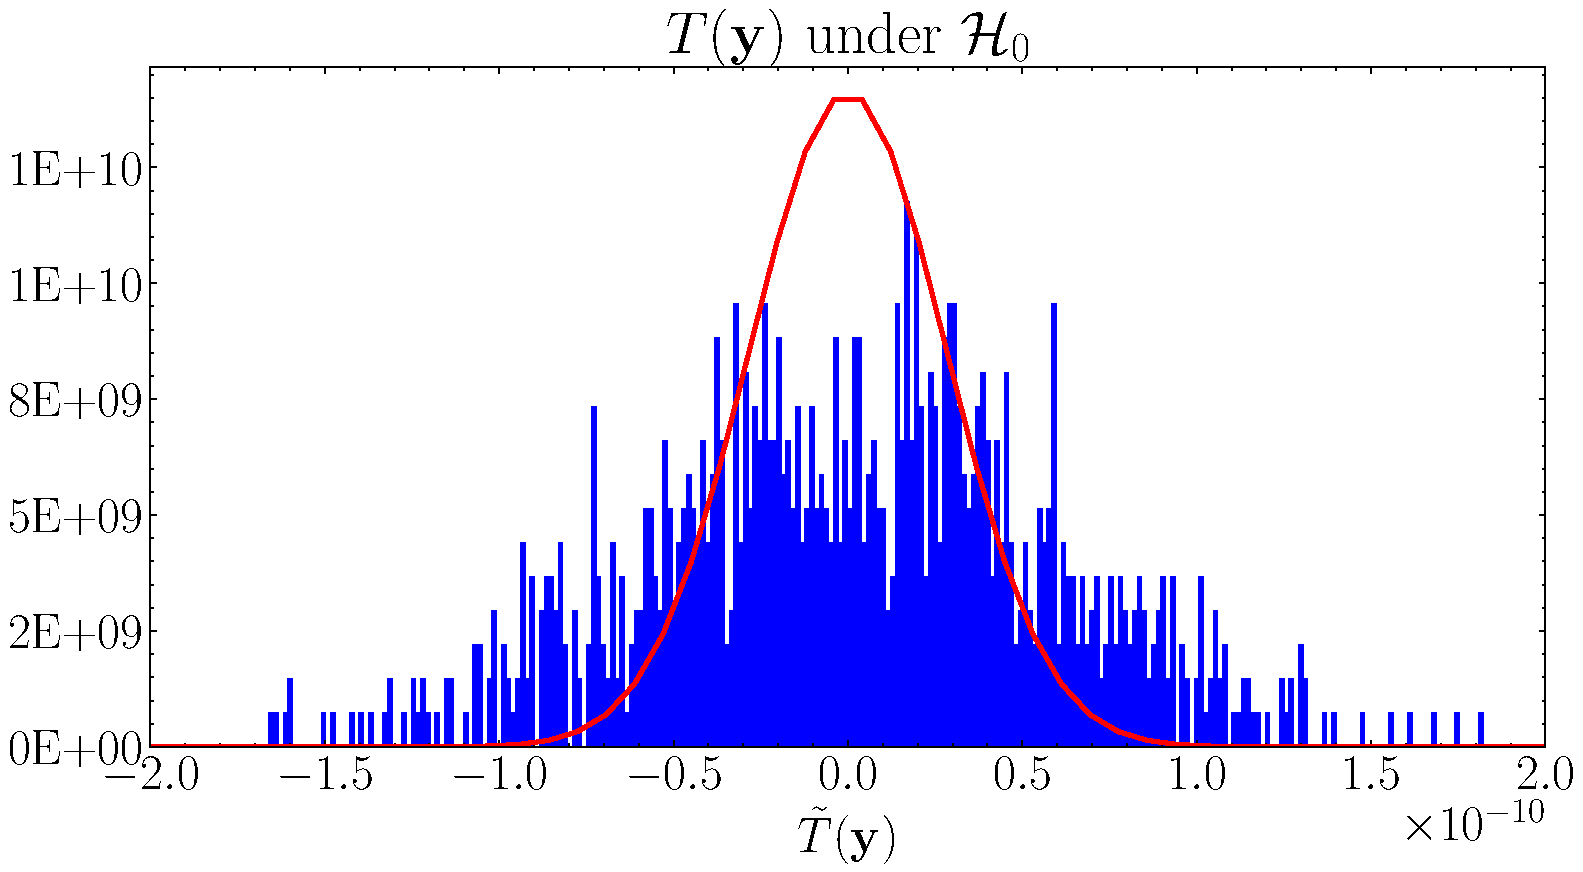
\includegraphics[width=3in]{../results/cycDist_H0I}}

\subfigure[Real component in $\cH_{1}$.]{\label{fig:CD_H1R}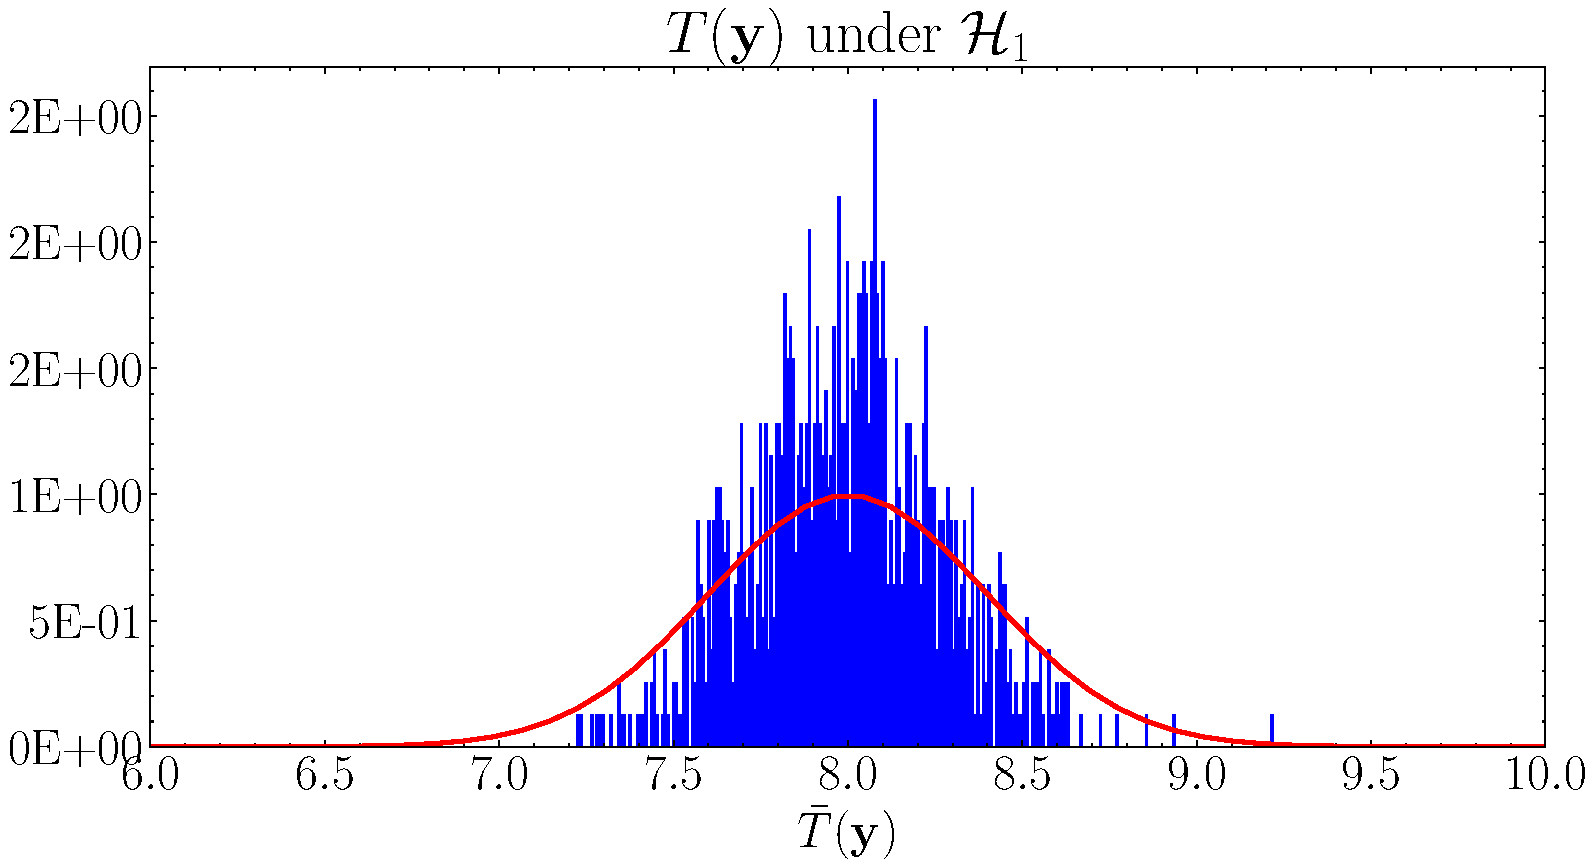
\includegraphics[width=3in]{../results/cycDist_H1R}}
\subfigure[Imaginary component in $\cH_{1}$.]{\label{fig:CD_H1I}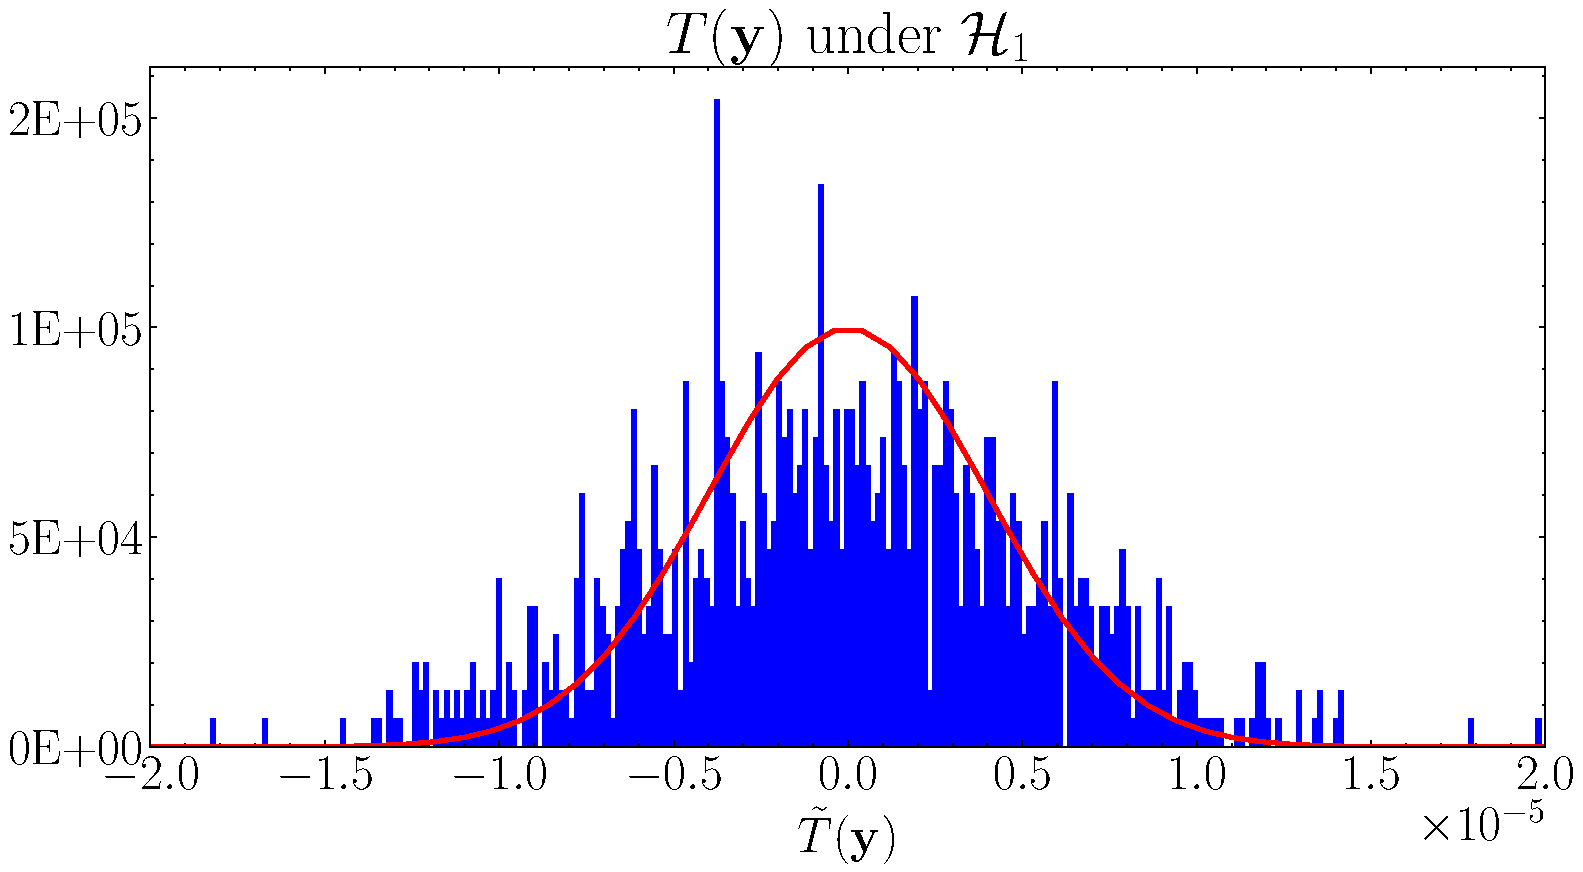
\includegraphics[width=3in]{../results/cycDist_H1I}}
\caption{Monte-Carlo distributions of the test statistics of the cyclostationary detector.}
\label{fig:CD_distributions}
\end{figure}

\noindent \linebreak {\it b) Monte-Carlo simulations with exact parameters:}

Figures \ref{fig:CDPD} and \ref{fig:CDPFA} shows the variation of $P_{D}$ and $P_{FA}$ with the signal-to-noise ratio (SNR). The estimated results are averaged over $1000$ realisations of the test statistic. The estimated probability and the theoretical probability match up to numerical precision. It can observed that the probability of detection increases monotonically with increase in SNR. As compared to the energy detector, the cyclostationary detector gives probability of detection $>0.9$ for SNR only $>-7$dB, which is $3$dB higher than the energy detector. However, the probability of false alarm is consistently, much lower than the probability of false alarm in the energy detector.
\begin{figure}[h]
\centering
\subfigure[Probability of detection.]{\label{fig:CDPD}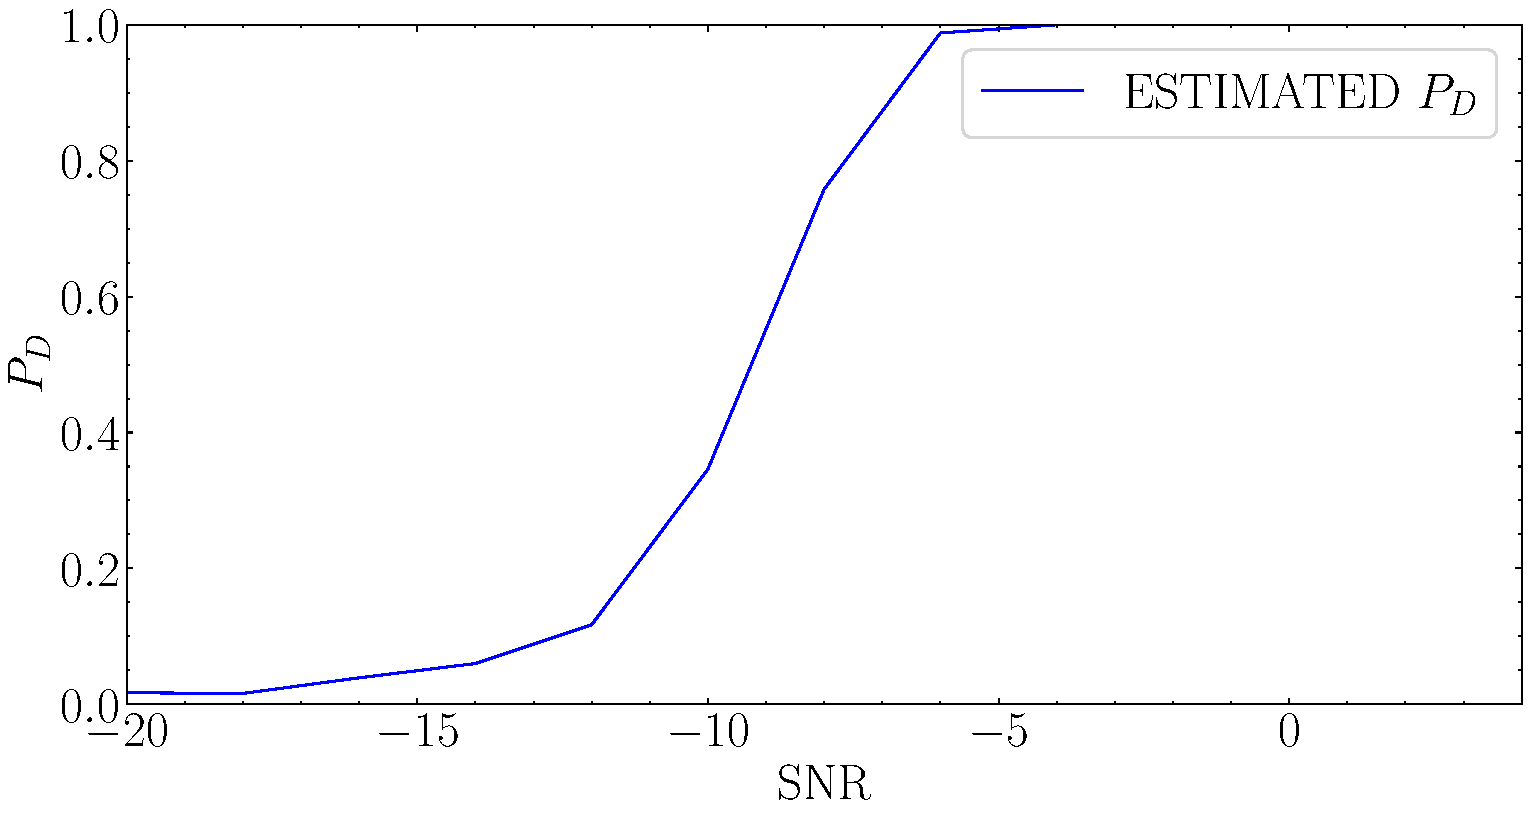
\includegraphics[width=3in]{../results/cycProb_PD}}
\subfigure[Probability of false alarm.]{\label{fig:CDPFA}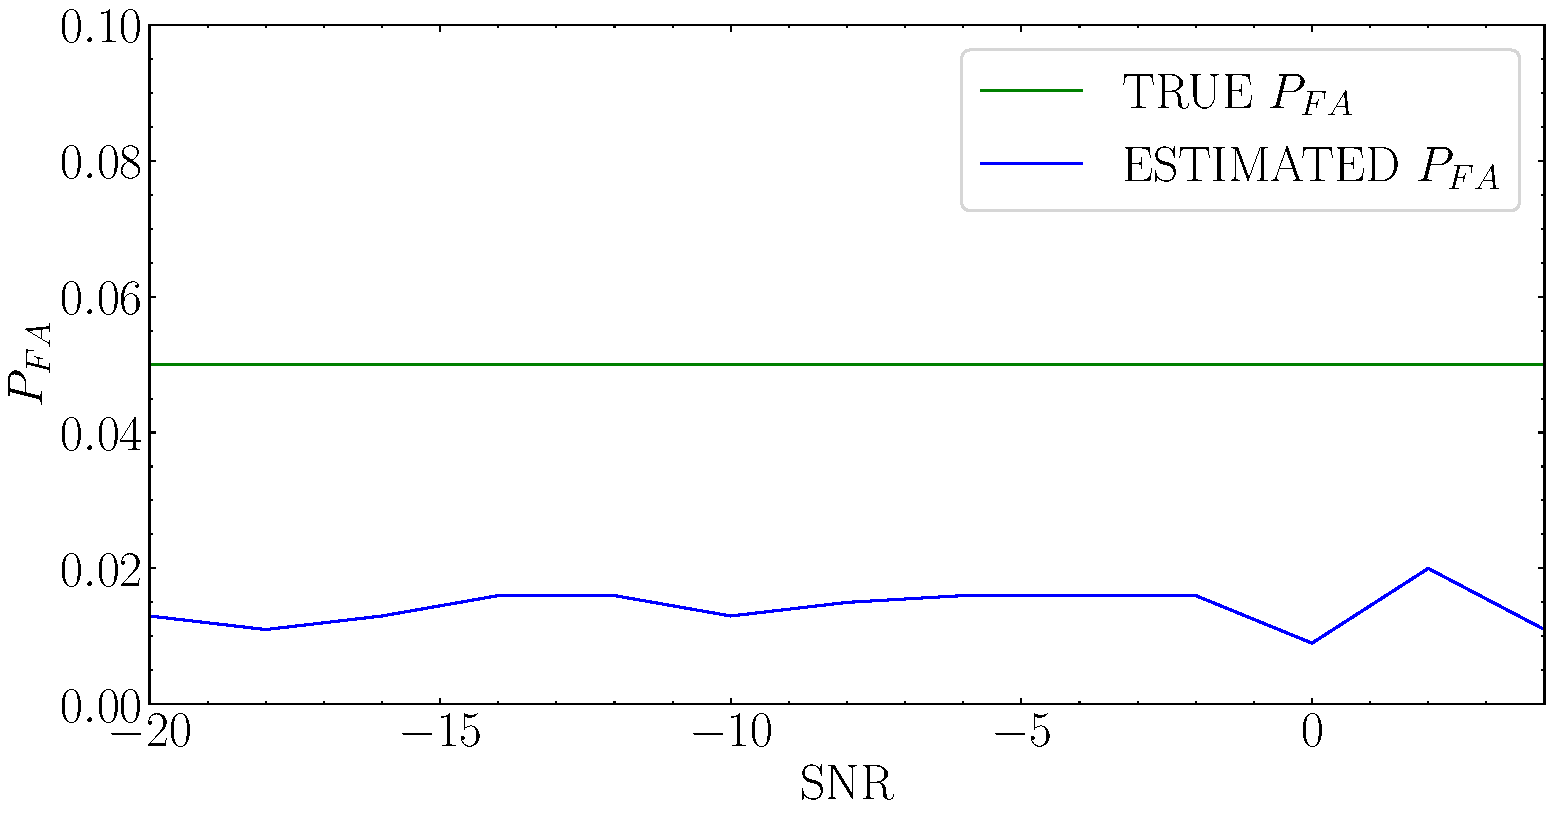
\includegraphics[width=3in]{../results/cycProb_PFA}}
\caption{Monte-Carlo probabilities of the cyclostationary detector varying with SNR when the parameters are exact.}
\label{fig:CD_exact}
\end{figure}

\noindent \linebreak {\it c) Monte-Carlo simulations with inexact parameters:}

Figures \ref{fig:CDPD_noise} and \ref{fig:CDPFA_noise} shows the variation of $P_{D}$ and $P_{FA}$ with the signal-to-noise ratio (SNR). The estimated results are averaged over $1000$ realisations of the test statistic. As compared to Figures \ref{fig:CDPD} and \ref{fig:CDPFA}, the probability of detection is only as high as $0.8$ at the SNR of $-7$dB. The probability of false alarm is marginally higher than in Figure \ref{fig:CDPFA}.
\begin{figure}[h]
\centering
\subfigure[Probability of detection.]{\label{fig:CDPD_noise}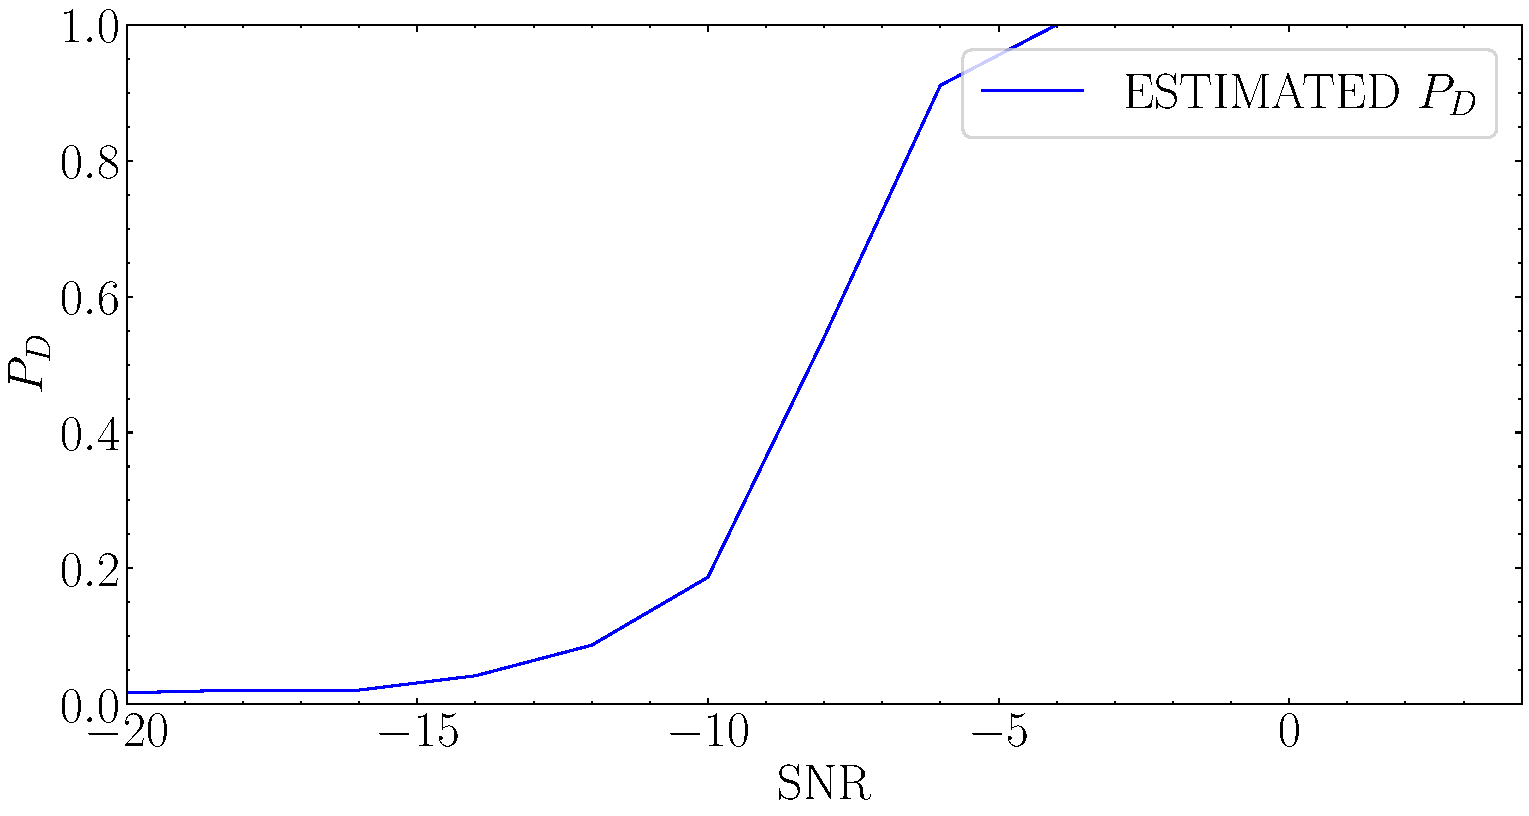
\includegraphics[width=3in]{../results/cycProb_PD_Noisy}}
\subfigure[Probability of false alarm.]{\label{fig:CDPFA_noise}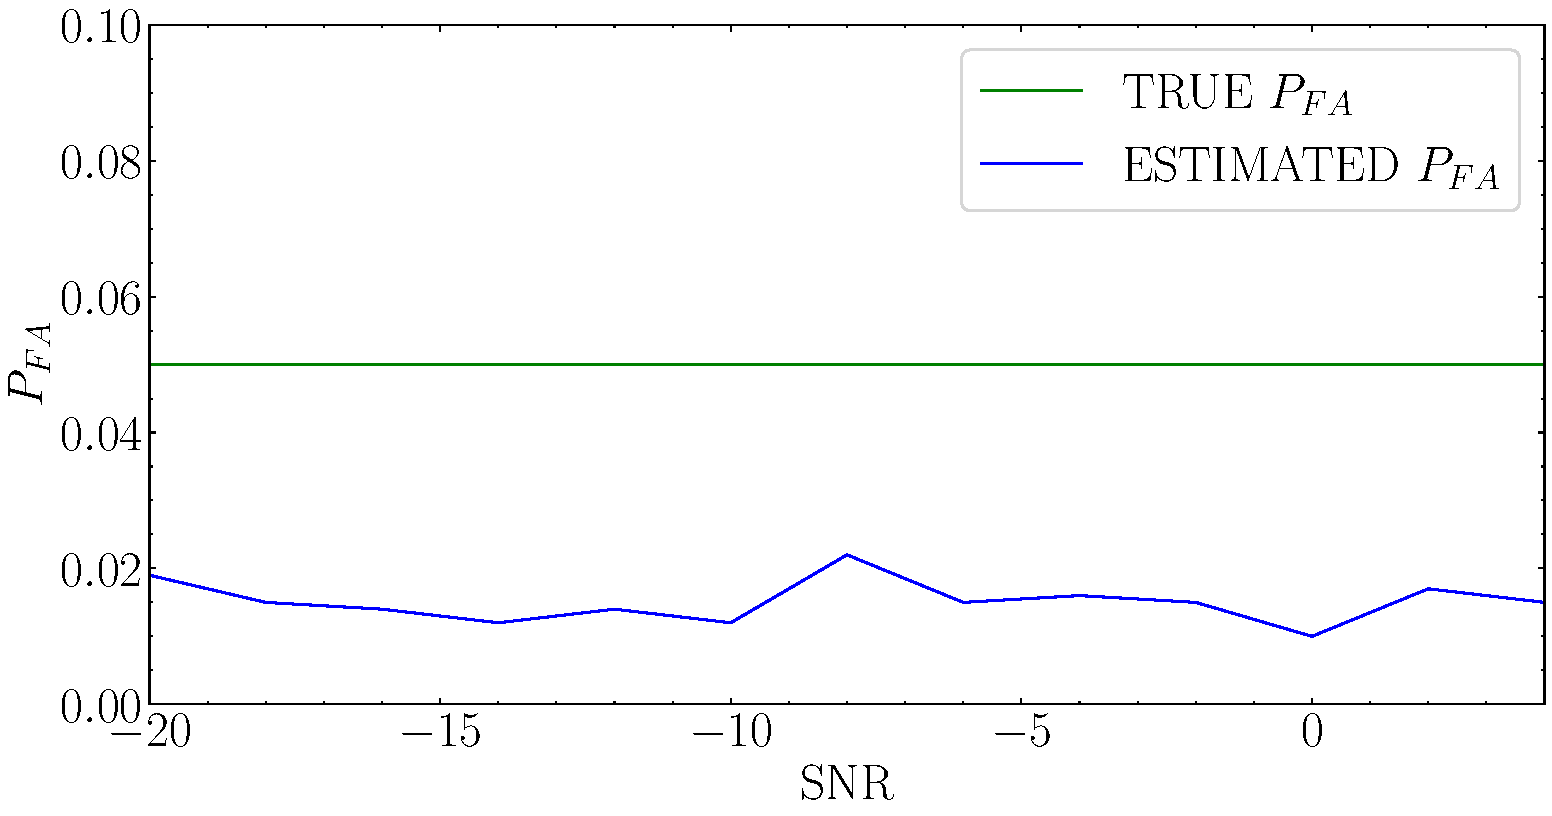
\includegraphics[width=3in]{../results/cycProb_PFA_Noisy}}
\caption{Monte-Carlo probabilities of the cyclostationary detector varying with SNR when the parameters are inexact.}
\label{fig:CD_inexact}
\end{figure}


% -----------------------------------------------------------------------------------------------------------------------
% -----------------------------------------------------------------------------------------------------------------------

%\appendix
%
%\subsection*{Scripts}
%
%The Python3 scripts to generate all figures can be downloaded from the GitHub repository \url{https://github.com/kamath-abhijith/Spectrum_Sensing}. Use \texttt{requirements.txt} to install all dependencies. Also, see the following code snippets for reference.
%
%\newpage
%\subsubsection*{Implementation of Interpolation using Wiener filter based methods}
%
%The relevant functions are in \texttt{utils.py}.
%\lstinputlisting[language=Python]{../interp_wiener.py}
%
%% -----------------------------------------------------------------------------------------------------------------------
%
%\subsubsection*{Implementation of Kalman Filter and Comparisons}
%
%The relevant functions are in \texttt{utils.py}.
%\lstinputlisting[language=Python]{../interp_kalman.py}
%
%% -----------------------------------------------------------------------------------------------------------------------
%
%\subsubsection*{\texttt{utils.py}}
%
%This script contains all the relevant functions and helpers.
%\lstinputlisting[language=Python]{../utils.py}

\end{document}
